\documentclass[aspectratio=169, lecture, amberg]{OTHAWbeamer}
\let\Tiny=\tiny  
\usepackage{ngerman}
\usepackage{amssymb}
\usepackage[utf8]{inputenc}
\usepackage{etex}
\usepackage{biblatex}
\usepackage{csquotes}
\usepackage{comment}
\usepackage{amsmath}
\usepackage{multirow}
\usepackage{makecell}
\usepackage{booktabs}
\usepackage{tabularx}

\usepackage{arydshln}


\addbibresource{references.bib}
\setbeameroption{show notes on second screen=right}
\setbeamerfont{note page}{size=\scriptsize}
\title[Forschungsseminar]{One-Step Image Translation with Text-to-Image Models}
\subtitle{Forschungsseminar}
\author[Schmidt]{Fabian Schmidt}
\place{OTH Amberg-Weiden}
\date{\today}

\email{f.schmidt3@oth-aw.de}

\begin{document}
\maketitle

% ---------- Begin Präsentation ----------
\frame{
\frametitle{Table of Contents}
\begin{enumerate}
    \item Introduction
    \item Related Work
    \item Terminology
    \item Method
    \item Experiments
    \item Discussion and Limitations
    \item Live Demo
\end{enumerate}
\tableofcontents
}

\begin{frame}
    \frametitle{Introduction}
    \framesubtitle{Problems with Diffusion Models}
    
    \begin{columns}
        \column{0.5\textwidth}
        \centering
        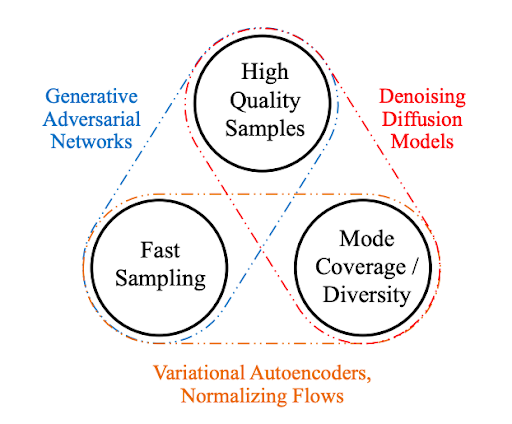
\includegraphics[width=0.9\textwidth]{images/GANs_Diffusion_Autoencoders.png}
    
        \column{0.5\textwidth}
        \centering
        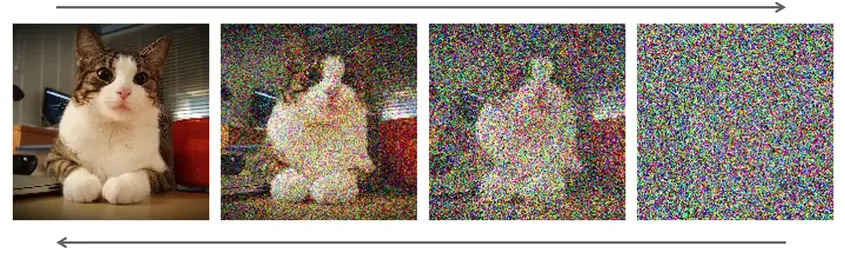
\includegraphics[width=\textwidth]{images/Generation-with-Diffusion-Models-ezgif.com-webp-to-jpg-converter.jpg}
      \end{columns}  
      \tiny{\footnotemark \url{https://developer.nvidia.com/blog/improving-diffusion-models-as-an-alternative-to-gans-part-1/}}
      \tiny{\footnotemark \url{https://miro.medium.com/v2/resize:fit:720/format:webp/1*RDPhd2dvmHE4UrAP-QHb9w.png}}
    \end{frame}
    \note{
        In dieser Arbeit werden zwei limitierende Faktoren von Diffusion Models angesprochen:\\
        \begin{itemize}
            \item Ihre lange Inference Zeit durch das Interative Denoising
            \item Die Notwendigkeit von Paired Daten
        \end{itemize}
    }
    
    % ---------- Proposed solutions ----------
    \begin{frame}
    \frametitle{Introduction}
    \framesubtitle{Proposed solutions}
    \begin{itemize}
        \item One-step image-to-image translation method for paired and unpaired settings
        \item Reduce number of inference steps to 1
        \item Trainable without image pairs
        \item Adapt pre-trained text-conditional one-step diffusion model to new domains via adversarial learning
    \end{itemize}
\end{frame}
\note{
    \begin{itemize}        
        \item Um das zu erreichen wird ein One-Step Image-to-Image Translation Ansatz vorgeschlagen, der sowohl in gepaarten als auch ungepaarten Einstellungen funktioniert.\\
        \item Dieser Ansatz reduziert die Anzahl der Inferenzschritte auf 1 und kann ohne Bildpaare trainiert werden.\\
        \item Außerdem kann ein vortrainiertes Text-Conditional One-Step Diffusion Model durch adversariales Lernen an neue Domänen angepasst werden.
        \item Es werden zwei Modelle traniert und mit bestehenden Methoden verglichen. 
        \item CycleGAN-Turbo für Unpaired Image-to-Image Translation
        \item Pix2Pix-Turbo für Paired Image-to-Image Translation
    \end{itemize}
}

\begin{frame}
    \frametitle{Related Work}
    \framesubtitle{Image-to-Image translation}
    Paired Image Translation
    \begin{itemize}
        \item e.g. GLIGEN \cite{li2023gligen}, T2I-Adapter \cite{mou2023t2i}, ControlNet \cite{zhang2023adding}
        \item requires large number of training pairs
        \item slow inference
    \end{itemize}
    Unpaired Image Translation
    \begin{itemize}
        \item GAN- or diffusion-based methods \cite{cyclediffusion} \cite{su2022dual} \cite{sasaki2021unitddpm}
        \item require training from scratch on new domains   
    \end{itemize}
\end{frame}
\note{
    \begin{itemize}
        
        \item Bei Image-to-Image translation versucht das Modell ein von einer source Domain in eine traget Domain zu übersetzen. Hierzu wird eine Kombination von reconstruction und adversarial loss verwendet.
        \item Aktuelle Arbeiten wie GLIGEN, T2I-Adapter und ControlNet bauen auf vortrainierten text-to-image modellen auf.
        \item Diese Methoden benötigen jedoch eine große Anzahl an Trainingsdaten und haben eine langsame Inferenzzeit.\\
        \item Es gibt auch Arbeiten die unpaired Image Translation verwenden. Diese Modelle basieren auf GANs oder Diffusion und benötigen ein komplettes retraining wenn sie auf neue Domains angewendet werden sollen.\\
        \item Was Paired und Unpaired Daten sind, kommt gleich. 
    \end{itemize}
    
    }
    
    % ---------- Text-to-Image models ----------
\begin{frame}
    \frametitle{Related Work}
    \framesubtitle{Text-to-Image models}
    \begin{itemize}
        \item Large-scale text-conditioned models have enhanced image quality and diversity by training on vast datasets \cite{schuhmann2022laion5b, kakaobrain2022coyo-700m}
        \item Zero-shot methods for editing real images use pre-trained text-to-image models, such as SDEdit \cite{meng2022sdedit}
        \item Despite impressive results, these methods face challenges in complex scenes with multiple objects.
    
    \end{itemize}
\end{frame}
\note{
    \begin{itemize}
        \item Große Text-to-Image Modelle haben gute Bildquilität und Vielfalt durch das Training auf rießigen Datensätzen.
        \item Zero-shot Methoden für die Bearbeitung von echten Bildern verwenden vortrainierte Text-to-Image Modelle wie SDEdit.        
        \item SDEdit bearbeitet reale Bilder, indem es dem Eingabebild Rauschen hinzufügt und es anschließend mit einem vorher trainierten Modell dem Prompt entsprechend entrauscht
        \item Trotz beeindruckender Ergebnisse haben diese Methoden Herausforderungen in komplexen Szenen mit mehreren Objekten.
        \item Bei den Experimenten wird das hier entwickelte Modell unteranderem mit SDEdit verglichen.
    \end{itemize}
}
    
% ---------- One-step generative models ----------
\begin{frame}
    \frametitle{Related Work}
    \framesubtitle{One-step generative models}
    To expedite diffusion model inference, recent works focus on:
    \begin{itemize}
        \item reducing the number of sampling steps using ODE solvers \cite{karras2022elucidating, lu2022dpmsolver}
        \item distilling slow multistep teacher models into fast few-step student models \cite{meng2022sdedit, salimans2022progressive}
        \item Using GANs directly for text-to-image synthesis \cite{kang2023scaling, sauer2023stylegant}
    \end{itemize}
    
    This work presents the first one-step conditional model that use both text and conditioning images.
\end{frame}
\note{
    \begin{itemize}
        \item Statt vielen denoising Schritten im Diffusion wird ein einziger Schritt verwendet.\\
        \item Andere Arbeiten verwenden ODE Solver um die Anzahl der Schritte zu reduzieren.\\
        \item Es gibt auch Arbeiten die langsame Modelle in schnelle Modelle umwandeln.\\
        \item GANs werden auch direkt für Text-to-Image Synthese verwendet.\\
        \item Diese Arbeit stellt das erste One-Step Conditional Model vor, das sowohl Text als auch Konditionierungs-Bilder verwendet.
        
    \end{itemize}
    
}

\begin{frame}
    \frametitle{Terminology}
    \framesubtitle{Generative Adversarial Networks(GAN)}
    \begin{figure}
        \centering
        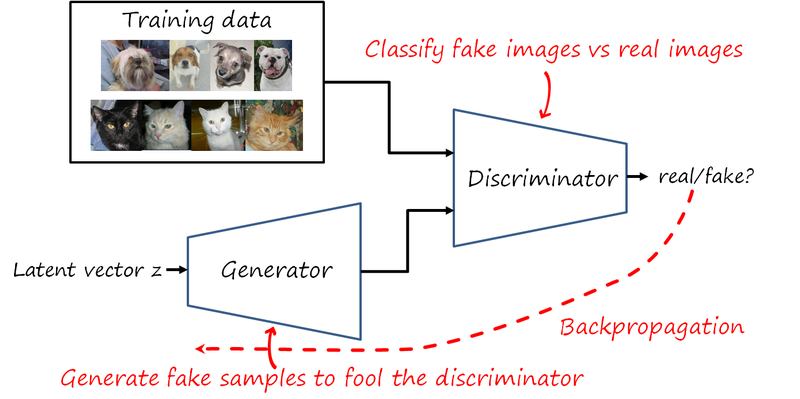
\includegraphics[width=0.65\linewidth]{images/blog_gan.png}
        \caption{GAN training process}
    \end{figure}
    \tiny{\footnotemark \url{http://www.lherranz.org/2018/08/07/imagetranslation/}}
\end{frame}
\note{}
    
% ---------- CycleGAN ----------
\begin{frame}
    \frametitle{Terminology}
    \framesubtitle{CycleGAN}
    \begin{figure}
        \centering
        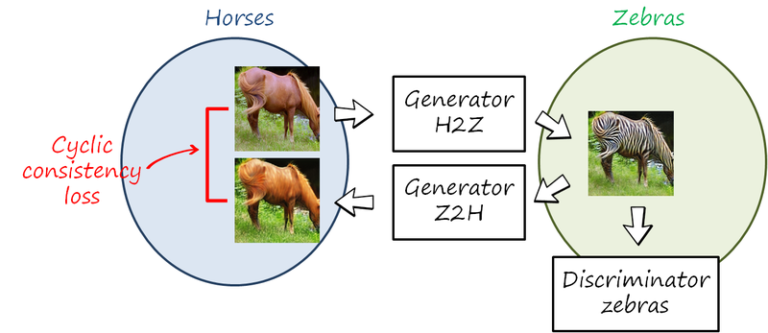
\includegraphics[width=0.78\linewidth]{images/blog_cyclegan_h2z2h-768x333.png}
        \caption{CycleGAN Architecture}
    \end{figure}
    \tiny{\footnotemark \url{http://www.lherranz.org/2018/08/07/imagetranslation/}}
\end{frame}
    
    
        
% ---------- UNet and Skip Connections ----------
\begin{frame}
    \frametitle{Terminology}
    \framesubtitle{UNet and Skip Connections}
    \begin{figure}
        \centering
        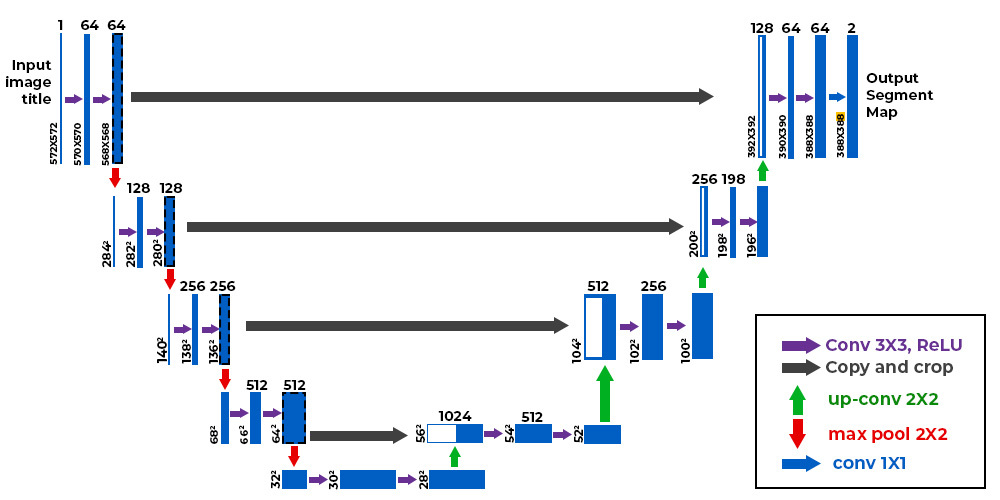
\includegraphics[width=0.6\linewidth]{images/Group14.jpg}
        \caption{Architecture}
    \end{figure}
\end{frame}
\note{
    \begin{itemize}
        \item UNet: Convolutional Neural Network, das für Bildsegmentierung verwendet wird
        \begin{itemize}
            \item Encoder Pfad: Mehrere Blöcke von convolutional layers mit ReLU activation und max pooling. Reduziert die Dimensionalität des Inputs
            \item Decoder Pfad: Mehrere Blöcke von convolutional layers mit RelU activation und upconvolution. Erhöht die Dimensionalität des Inputs. Außerdem Concatenation mit entsprechenden Encoder Pfad
            \item Skip Connections: Verbindung zwischen Encoder und Decoder Pfad. Hilft details zu erhalten, die im Encoder verloren gehen würden
        \end{itemize}
    \end{itemize}
}
    
% ---------- LoRA Weights ----------
\begin{frame}
    \frametitle{Terminology}
    \framesubtitle{LoRA Weights}
    \begin{figure}
        \centering
        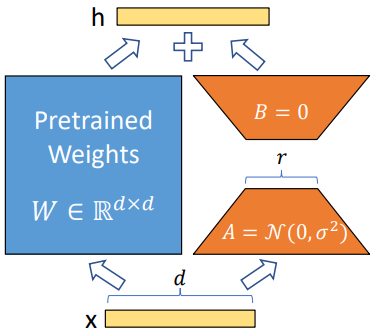
\includegraphics[width=0.4\linewidth]{images/Bildschirmfoto vom 2024-04-15 10-21-59.png}
        \caption{\textbf{Lo}w \textbf{R}ank \textbf{A}daption}
    \end{figure}
\end{frame}

% ---------- Paired vs unpaired data ----------
\begin{frame}
\frametitle{Terminology}
\framesubtitle{Paired vs unpaired data}
\begin{columns}
    \column{0.5\textwidth}
    \centering    
    \begin{figure}
        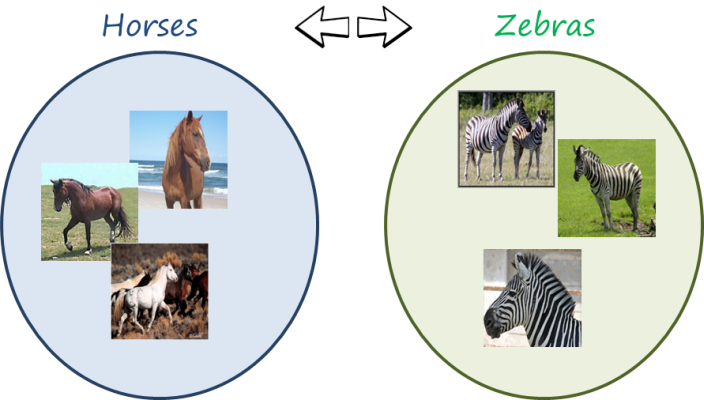
\includegraphics[width=0.75\textwidth]{images/blog_unpairedimagetranslation2.png}
        \caption{Unpaired Data}
    \end{figure}

    \column{0.5\textwidth}    
    \centering    
    \begin{figure}        
        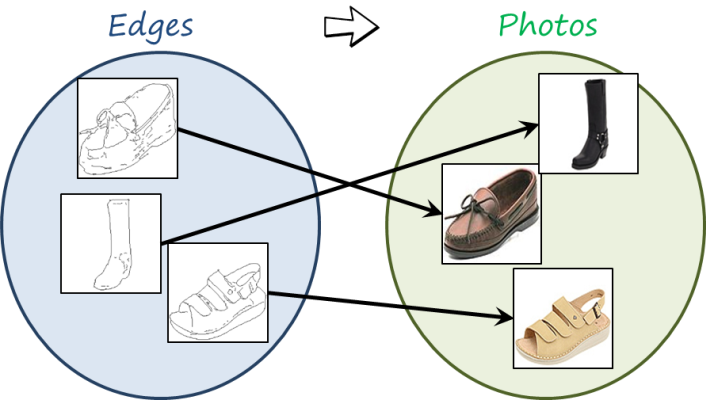
\includegraphics[width=0.75\textwidth]{images/blog_pairedimagetranslation.png}
        \caption{Paired Data}
    \end{figure}
    \end{columns}
\end{frame}
\note{
    \begin{itemize}
        \item Paired data: Jedes Bild in Domain X hat ein korrespondierendes Bild in Domain Y
        \item Unpaired data: Es gibt keine direkte Zuordnung zwischen den Bildern in Domain X und Domain Y
    \end{itemize}

}


\begin{frame}
\frametitle{Method}
\framesubtitle{Adding Conditioning Input}
\begin{figure}
    \centering
    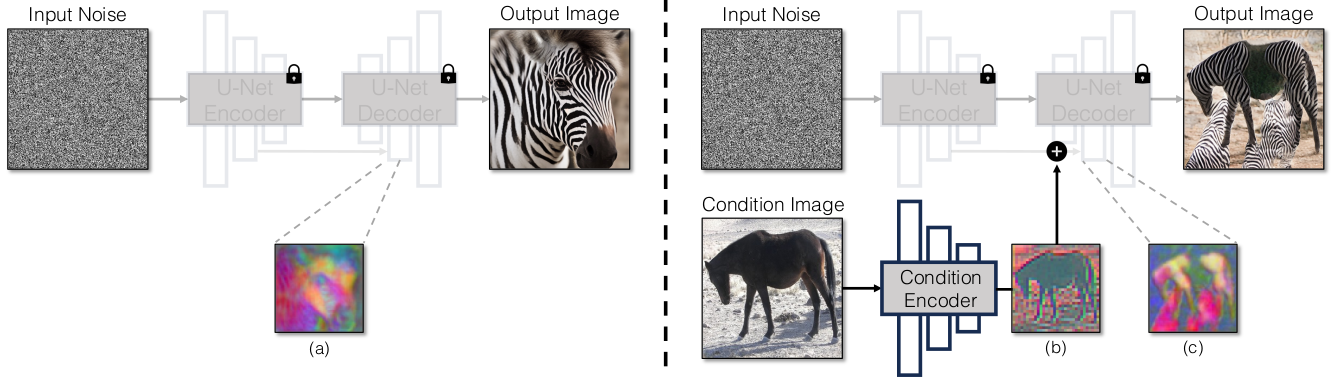
\includegraphics[width=1\linewidth]{images/Bildschirmfoto vom 2024-04-14 10-57-39.png}
    \caption{Conflicts between noise and conditional input}
\end{figure}
\end{frame}
\note{
    Methoden-Teil:\\
    \begin{enumerate}
        \item Begonnen wird mit einem one-step pre-trained text-to-image Model, welches realistische Bilder erzeugen kann, hier Stable Diffusion Turbo        
        \item Text-to-image Modelle zu einem Image-Translation Modell umwandeln
        \item Problem von detail verlust bei der Übersetzung wie das umgangen werden kann
        \item Unpaired image translation
        \item Architecture Änderungen für Paired image Translation
    \end{enumerate}
    
    \textbf{RESTLICHEN NOTIZEN SIEHE ZETTEL}
    
}

% ---------- Preserving Input Details ----------
\begin{frame}
\frametitle{Method}
\framesubtitle{Preserving Input Details}
\begin{figure}
    \centering
    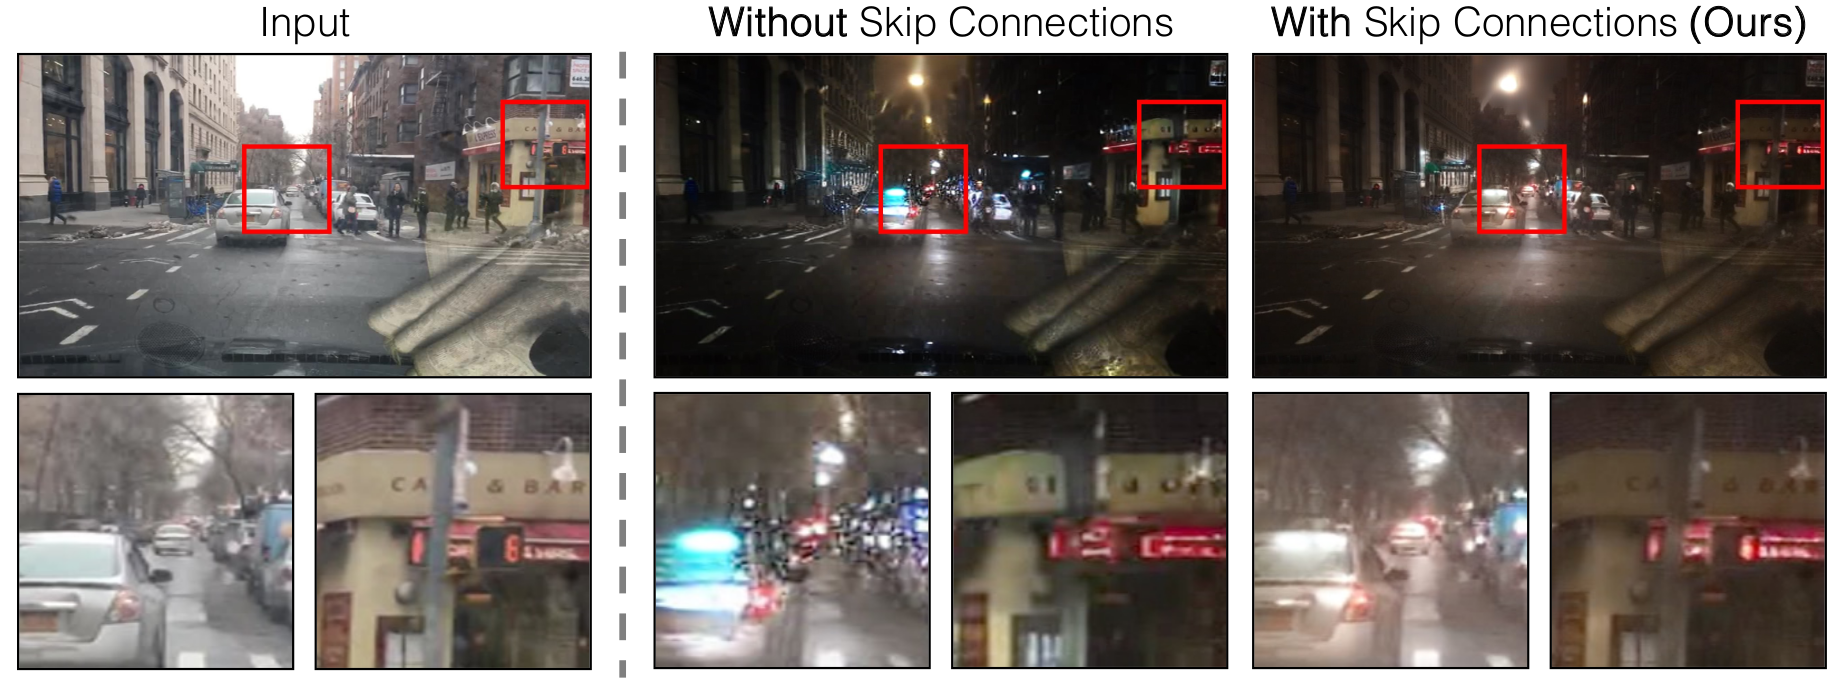
\includegraphics[width=0.9\linewidth]{images/Bildschirmfoto vom 2024-04-14 11-06-40.png}
    \caption{Skip Connections help retain details}
\end{figure}
\end{frame}
\note{
    Warum gehen Details verloren?\\
    \begin{itemize}
        \item Die Bild Encoder von Latent Diffusion Modellen komprimieren Inputbilder um das 8fache und erhöhen die Dimension von 3 auf 4
        \item So wird zwar Training und Inference von Diffusion Modellen schneller, ist aber nicht ideal für Image Translation, wo man details erhalten will
    \end{itemize}
    Wie können Details erhalten werden?\\
    \begin{itemize}
        \item Um Details zu erhalten werden Skip Connections zwischen Encoder und Decoder eingeführt
        \item Nach jedem Downsampling Schritt im Encoder wird eine 1x1 zero-convolution schicht durchlaufen und an die entsprechende Schicht im Decoder weitergegeben
    \end{itemize}
    Siehe Bild, links der Input, Mitte ohne Skip Connections, rechts mit Skip Connections\\
    Ohne Skip Connections verschwindet das Auto in der Ferne und der Text ist nicht lesbar
}


% ---------- Preserving Input Details ----------
\begin{frame}
\frametitle{Method}
\framesubtitle{Preserving Input Details}
\begin{figure}
    \centering
    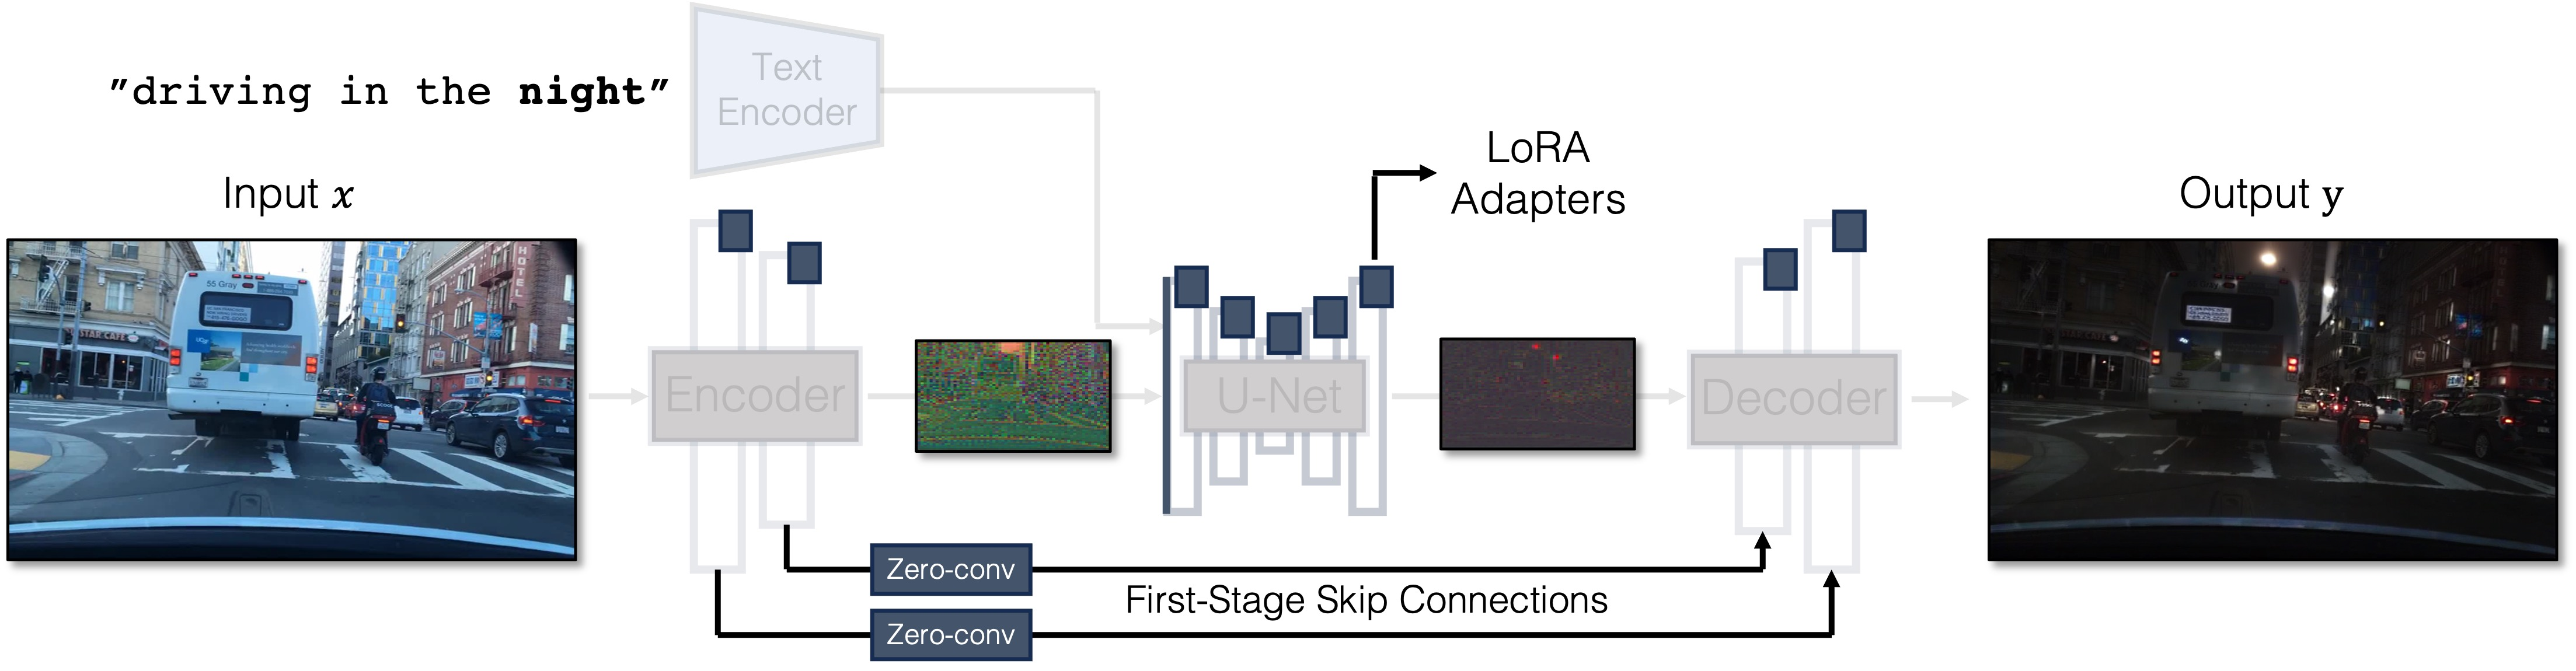
\includegraphics[width=1\linewidth]{images/method.jpg}
    \caption{Model Architecture}
\end{figure}
\end{frame}
\note{
    Die Architecture besteht im wesentlichen aus 4 Teilen:
    \begin{enumerate}
        \item Einem Text Encoder und einem Bild Encoder für den Input
        \item Das vortrainierte Stable Diffusion Model
        \item Und einem Decoder
        \item Der Text Encoder, Bild Encoder und Decoder stammen alle aus dem StableDiffuion Model
        \item In das Model und dem Encoder und Decoder wurden auf jeder Ebene LoRA Gewichte eingeführt
        \item Die erste schicht des Stable Diffusion wird neu trainiert
        \item Und es werden 1x1 zero-convolution Skip Connecitons zwischen Encoder und Decoder eingeführt
        \item Kurz gesagt, alles was Blau ist wurde neu trainiert, alles was grau ist bleibt unverändert
    \end{enumerate}
}


% ---------- Unpaired Training ----------
\begin{frame}
    \frametitle{Method}
    \framesubtitle{Unpaired Training}
    \begin{align*}
    \text{Goal:} &\text{ Convert images from } \mathcal{X} \subset \mathbb{R} ^{H \times W \times 3} \
    \text{ to } \mathcal{Y} \subset \mathbb{R} ^{H \times W \times 3} \\
    &\text{ given an unpaired dataset } \mathcal{X} = {x \in \mathcal{X} } \text{ and } \mathcal{Y} = {y \in \mathcal{Y} } \\
    &\text{ using one network } G \text{ and two translations } G(x, c_y): \mathcal{X} \rightarrow \mathcal{Y} \
    \text{ and } G(y, c_x): \mathcal{Y} \rightarrow \mathcal{X}
    \end{align*}
\end{frame}
\note{
    Ziel ist es Bilder von der Domain X in Domain Y zu übersetzen.\\
    Bei zwei gegebenen unpaired Datensätzen X und Y\\
    Und das ganze mit dem gleichen Netzwerk G\\
    Die Notation $G(x,c_y)$ bedeutet, dass das Netzwerk x in y übersetzt, wobei $c_y$ eine Übersetzungsaufgabe darstellt z.B. Tag -> Nacht
}


\begin{frame}
\frametitle{Method}
\framesubtitle{Unpaired Training}
\begin{block}{Cycle consistency with perceptual loss}
    \begin{equation}
        \mathcal{L}_{\text{cycle}}(G, F) = \mathbb{E}_x [ \mathcal{L}_\text{rec} (G(G(x,c_Y), c_X), x) ] + \mathbb{E}_y [ \mathcal{L}_\text{rec} (G(G(y,c_X), c_Y), y) ]
    \end{equation}
\end{block}
with $\mathcal{L}_{\text{rec}}$ as combination of L1 and LPIPS \cite{zhang2018unreasonable}
\begin{block}{Adversarial loss}
    \begin{align}
        \mathcal{L}_{\text{GAN}} &= \mathbb{E}_{y} [\log D_Y(y)] + \mathbb{E}_{x} [\log(1 - D_Y(G(x,c_Y)))] \\
        &+ \mathbb{E}_{x} [\log D_X(x)] + \mathbb{E}_{Y} [\log(1 - D_X(G(y,c_X)))]
    \end{align}
\end{block}
\end{frame}
\note{
    Cycle Consistency loss: \\
    \begin{itemize}
        \item Die Cycle Consistency Loss Funktion sorgt dafür, dass die Übersetzung von x nach y und wieder zurück das Originalbild x ergibt
        \item $\mathcal{L}_{\text{rec}}$ ist eine Kombination aus L1 und LPIPS Loss
        \item LPIPS steht für Learned Perceptual Image Patch Similarity und ist ein Maß für die Ähnlichkeit von Bildern. Das Maß ist vergleichbar mit menschlicher Wahrnehmung

    \end{itemize}
    Adversarial loss: \\
    \begin{itemize}
        \item Der Adversarial loss sorgt dafür, dass die Übersetzung von x nach y bzw. von y nach x möglichst der Ziel Domain entspricht.
        \item Hier zu werden zwei Discriminatoren $D_x$ und $D_y$, um Übersetzte Bilder von Realen zu unterscheiden
        \item Die Discriminatoren nutzen hierfür beide das CLIP Modell(Contrastive Language-Image Pre-training)
    \end{itemize}
}


\begin{frame}
\frametitle{Method}
\framesubtitle{Unpaired Training}
\begin{block}{Identity regularization loss}
    \begin{equation}
        \mathcal{L} _{\text{idt}} = \mathbb{E} _y [ \mathcal{L}_{\text{rec}}(G(y,c_Y),y)] + \mathbb{E}_x [ \mathcal{L}_{\text{rec}}(G(x,c_X),x)]
    \end{equation}
\end{block}


\begin{block}{Full objective}
    \begin{equation}
        \arg \underset{G}{\min} \mathcal{L}_{\text{cycle}} + \lambda _{\text{idt}} \mathcal{L}_{\text{idt}} + \lambda_{\text{GAN}}\mathcal{L}_{\text{GAN}}
    \end{equation}
\end{block}
\end{frame}
\note{
    Identity Regularization loss: hilft dabei, dass Inhalte aus dem Inputbild bei der Übersetzung nicht verloren gehen.\\
    Full Objective: Die Gesamtverlustfunktion setzt sich aus den drei Verlustfunktionen zusammen.\\

}


% ---------- Extensions ----------
\begin{frame}
\frametitle{Method}
\framesubtitle{Extensions - Paired Training}
\begin{itemize}
    \item Adaptation of network G to paired setting, like edge-to-image or sketch-to-image, called pix2pix-Turbo
    \item new translation function $G(x,c): X \rightarrow Y$ where $X$ is source domain, $Y$ target domain and $c$ conditioning input
\end{itemize}
\begin{block}{Loss Function}
    \begin{equation}
        \arg \underset{G}{\min} \mathcal{L}_{\text{rec}}+ \lambda _{\text{clip}}\mathcal{L}_{\text{CLIP}}+ \lambda_{\text{GAN}}\mathcal{L}_{\text{GAN}}
    \end{equation}
\end{block}
\end{frame}
\note{
    Der Fokus des Papers liegt zwar auf unpaired Image Translation, aber es gibt auch eine Erweiterung für paired Image Translation.\\
    Dieser Abschnitt befasst sich mit der Anpassung des Netzwerks G an ein gepaartes Setting, wie z.B. Kanten-zu-Bild oder Skizze-zu-Bild, genannt pix2pix-Turbo.\\
    Die neue Übersetzungsfunktion $G(x,c): X \rightarrow Y$ wobei $X$ die Quelldomäne, $Y$ die Ziel-Domäne und $c$ die Konditionierungseingabe ist.\\
    Die neue Verlustfunktion setzt sich aus der Rekonstruktionsverlustfunktion, dem CLIP text-image alignment Verlust und dem GAN-Verlust zusammen.\\
    GAN-Verlust und Rekonstruktionsverlust sind die gleichen wie im unpaired Setting\\
    CLIP text-image alignment Verlust ist ein Maß für die Ähnlichkeit von Bildern und Texten
}


\begin{frame}
    \frametitle{Method}
    \framesubtitle{Extensions - Generating diverse output}
    Introduction of interpolation coefficient $\gamma$ \newline 
    Three changes to the Architecture (1/3):
    \begin {itemize}
        \item Generator function $G(x,z,\gamma)$ combines noise z and encoder output like so: $\gamma G_{\text{enc}}(x) + (1 - \gamma) z$
        \item Output as U-Net input
    \end{itemize}
\end{frame}
\note{
    Zur Generierung von diversen outputs wir eine Interpolationskoeffizient $\gamma$ eingeführt.\\
    Desweiteren werden drei Änderungen an der Architektur vorgenommen.\\
    1. $gamma$ wird in die Generatorfunktion eingeführt.\\
    2. Der Output wird als U-Net Input verwendet
}


\begin{frame}
    \frametitle{Method}
    \framesubtitle{Extensions - Generating diverse output}
    Three changes to the Architecture (2/3):
    \begin {itemize}
        \item Scale LoRA weights and skip connections according to $\theta = \theta_0 + \gamma \Delta \theta$  
        \item where $\theta_0$ and $\Delta \theta$ denote the original weights and new weights.
    \end{itemize}
\end{frame}
\note{
    Skalierung von LoRA Gewichte und Outputs von Skip Connections neu gewichten
}


\begin{frame}
    \frametitle{Method}
    \framesubtitle{Extensions - Generating diverse output}
    Three changes to the Architecture (3/3):
    \begin {itemize}
        \item Scale reconstruction loss according to $\gamma$: $\mathcal{L}_{\text{diverse}} = \mathcal{L}_{x,y,z,\gamma} \gamma\mathcal{L}_{\text{rec}}(G(x,z,\gamma),y)]$
        \item $\gamma = 0$ corresponds to default stochastic behavior of pretrained model, in this case reconstruction loss is not enforced
        \item $\gamma = 1$ corresponds to deterministic translation from previoues seections
    \end{itemize}
\end{frame}
\note{
    Rekonstruktionsverlust wird nach $\gamma$ skaliert.\\
    $\gamma = 0$ entspricht dem Standardverhalten des vortrainierten Modells, in diesem Fall wird der Rekonstruktionsverlust nicht durchgesetzt.\\
    $\gamma = 1$ entspricht der deterministischen Übersetzung aus den vorherigen Abschnitten
}


\begin{frame}
\frametitle{Experiments - Paired Image Translation}
\framesubtitle{Baselines}
Training details:
\begin{itemize}
    \item 330MB of trainable parameters for unpaired models(LoRA weights, zero-conv layer, first conv layer of U-Net)
    \item Adam Optimizer with learning rate: 1e-6, batch size:8, $\lambda _{\text{idt}} = 1$, $\lambda _{\text{GAN}} = 0.5$
\end{itemize}
Datasets:
\begin{table}
    \centering
    \begin{tabular}{|c|c|c|c|}
        Task & Images Source & Images Target & Dataset \\
        \hline
        Horse $\leftrightarrow$ Zebra & 939 & 1177 & ImageNet \cite{5206848}\\
        Winter $\leftrightarrow$ Summer & 854 & 1273 & Flickr \cite{zhu2020unpaired} \\
        Day $\leftrightarrow$ Night & Day subset & Night subset & BDD100k \cite{yu2020bdd100k}\\
        Clear $\leftrightarrow$ Foggy & 12454 & 572 & BDD100k and DENSE \cite{bijelic2020seeing}
    \end{tabular}       
\end{table}
\end{frame}
\note{    
    \textbf{Erstens}: Vergleich mit diversen GAN- und Diffusion Modellen\\
    \textbf{Zweitens}: Analyse der verschiedenen Komponenten des Modells\\
    \textbf{Drittens}: Vergleich mit unpaired Methoden
    
    \begin{itemize}
        \item 330MB an trainierbaren Parametern, mit LoRA Gewichten, Zero-Conv Layer und erster Conv Layer des U-Net
        \item Adam Optimizer mit Lernrate: 1e-6, Batch-Size: 8, $\lambda _{\text{idt}} = 1$, $\lambda _{\text{GAN}} = 0.5$
        \item Horse $\leftrightarrow$ Zebra und Winter $\leftrightarrow$ Summer sind 286x286, hier wird zufällig auf 256x256 gecroppt. In Inference wird die Tranformation auf 256x256 durchgeführt.
        \item Day $\leftrightarrow$ Night und Clear $\leftrightarrow$ Foggy, hier wird auf 512x512 resized für training und Inference.
        \item Für Evaluation wird das zugehörige Validation-Set verwendet.4
    \end{itemize}

}

\begin{frame}
    \frametitle{Experiments - Paired Image Translation}
    \framesubtitle{Baselines}
    Evaluation Protocol:
    \begin{itemize}
        \item match data distribution of target domain $\rightarrow$ FID \cite{heusel2018gans}
        \item preserve input image structure in translated output $\rightarrow$ DINO \cite{tumanyan2022splicing}
        \item Inference runtime using a single NVIDIA RTX A6000 GPU
        \item human preceptual study
    \end{itemize}
\end{frame}
\note{
    Zwei wesentliche Ziele für Image Translation Modelle:\\
    \textbf{Erstens}: Die Verteilung der Ziel Domain möglichst gut matchen -> FID Score Frechet Inception Distance. Misst den Unterschied zwischen zwei Image sets (echt und fake). Basiert auf der Frechet Distance zwischen Zwei Wahrscheinlichkeitsverteilungen\\
    \textbf{Zweitens}: Die Struktur des Eingabebildes im übersetzten Bild erhalten -> DINO structural Distillation\\
    \begin{itemize}
        \item Ein niedriger FID Score zeigt einen guten Match zwichen der Verteilung der Ziel Domain und der generierten Bilder
        \item Ein niedriger DINO Score zeigt, dass die Struktur des Eingabebildes im übersetzten Bild erhalten bleibt
        \item niedriger FID und hoher DINO Score heißt, dass die Struktur des Eingabebildes im übersetzten Bild nicht erhalten bleibt
        \item hoher FID und niedriger DINO Score heißt, dass das Eingabebild kaum verändert wird -> Beide Scores betrachten
        \item zusätzlich wird die Inferenzzeit auf einer NVIDIA RTX A6000 GPU gemessen 
    \end{itemize}
}

% ---------- Comparison to Unpaired Methods ----------
\begin{frame}
    \frametitle{Experiments - Paired Image Translation}
    \framesubtitle{Comparison to Unpaired Methods}
    \begin{figure}
        \centering
        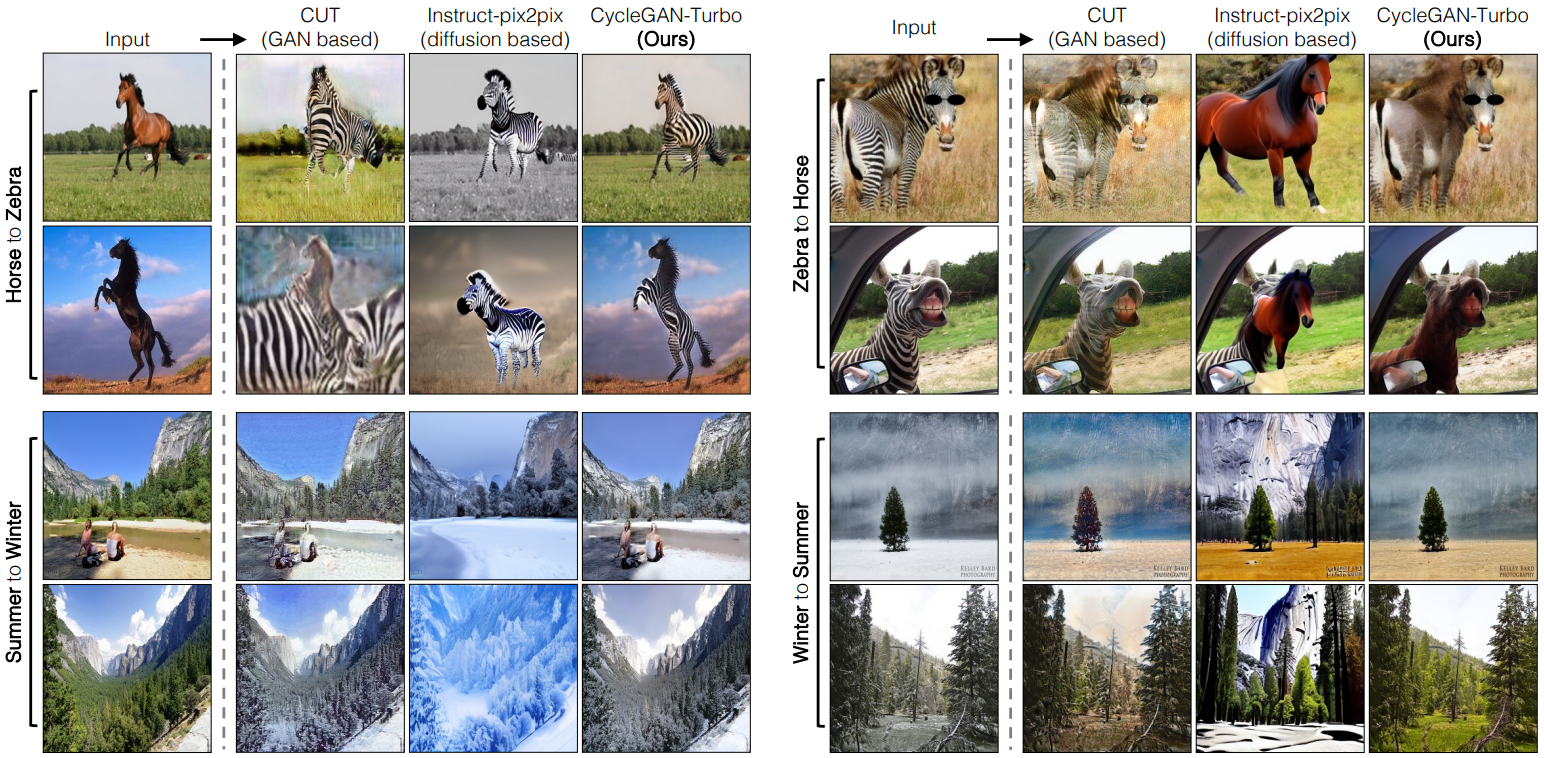
\includegraphics[width=0.85\linewidth]{images/horse_zebra.png}
        
    \end{figure}
\end{frame}
\note{
    Zuerst für die Tasks Horse $\rightarrow$ Zebra und Zebra $\rightarrow$ Horse und Winter $\rightarrow$ Summer und Summer $\rightarrow$ Winter
    \begin{itemize}
        \item Hier nur die Outputs für ein GAN-Modell und ein Diffusion-Modell. Für die Outputs der anderen Modelle für die Horse $\leftrightarrow$ Zebra Task verweise ich auf Anhang C im Paper
        \item Für die GAN-Modelle werden default Hyperparameter verwendet und auf allen Datensets für 100k Iterationen trainiert
    \end{itemize}
}




\begin{frame}
    \frametitle{Experiments - Paired Image Translation}
    \framesubtitle{Comparison to Unpaired Methods}
   
    \begin{table}
        \centering
    
     \vspace{-5pt}
        \resizebox{\linewidth}{!}{
        \begin{tabular}{l c cc cc cc cc}
            \toprule 
            \multirow{3}{*}{\textbf{Method}} 
            & \multirow{3}{*}{\textbf{\shortstack[c]{Infrence \\ time }}} 
            & \multicolumn{2}{c}{\textbf{Horse $\rightarrow$ Zebra} }
            & \multicolumn{2}{c}{\textbf{Zebra $\rightarrow$ Horse} }
            & \multicolumn{2}{c}{\textbf{Summer $\rightarrow$ Winter} }
            & \multicolumn{2}{c}{\textbf{Winter $\rightarrow$ Summer} }
            \\
    
            \cmidrule(lr){3-4} \cmidrule(lr){5-6} \cmidrule(lr){7-8} \cmidrule(lr){9-10} 
            &
            & \multirow{2}{*}{\shortstack[c]{FID $\downarrow$ }}  
            & \multirow{2}{*}{\shortstack[c]{DINO \\ Struct. $\downarrow$ }} 
    
            & \multirow{2}{*}{\shortstack[c]{FID $\downarrow$ }}  
            & \multirow{2}{*}{\shortstack[c]{DINO \\ Struct. $\downarrow$ }} 
    
            & \multirow{2}{*}{\shortstack[c]{FID $\downarrow$ }}  
            & \multirow{2}{*}{\shortstack[c]{DINO \\ Struct. $\downarrow$ }} 
    
            & \multirow{2}{*}{\shortstack[c]{FID $\downarrow$ }}  
            & \multirow{2}{*}{\shortstack[c]{DINO \\ Struct. $\downarrow$ }} 
            
            \\ \\
            \cmidrule(lr){1-10}
    
            CycleGAN \cite{zhu2020unpaired}  & 0.01s
            & 74.9 & 3.2 
            & 133.8 & 2.6
            & 62.9 & 2.6
            & 66.1 & 2.3 
            \\
            
            
            CUT \cite{park2020contrastive} & 0.01s
            & 43.9 & 6.6 
            & 186.7 & 2.5 
            & 72.1 & 2.1 
            & 68.5 & 2.1 \\
            
            \hdashline
    
            SDEdit \cite{meng2022sdedit} & 1.56s
            & 77.2 & 4.0
            & 198.5 & 4.6  
            & 66.1 & 2.1 
            & 76.9 & 2.1\\
            
            Plug\&Play \cite{tumanyan2022plugandplay} & 7.57s
            & 57.3 & 5.2  
            & 152.4 & 3.8 
            & 67.3 & 2.8 
            & 73.3 & 2.6\\
            
            Pix2Pix-Zero \cite{parmar2023zeroshot}  & 14.75s
            & 81.5 & 8.0
            & 147.4 & 7.8
            & 68.0 & 3.0
            & 93.4 & 4.3 \\
            
            Cycle-Diffusion \cite{cyclediffusion} & 3.72s
            & \textbf{38.6} & 6.0 
            & 132.5 & 5.8 
            & 64.1 & 3.6
            & 70.3 & 3.6 \\
    
            DDIB \cite{su2022dual} & 4.37s
            & 44.4 & 13.1  
            & 163.3 & 11.1 
            & 90.8 & 7.2
            & 88.9 & 6.8 \\
    
            InstructPix2Pix \cite{brooks2023instructpix2pix} & 3.86s
            & 51.0 & 6.8 
            & 141.5 & 7.0 
            & 68.3 & 3.7 
            & 85.6 & 4.4 \\
            \hdashline
    
            CycleGAN-Turbo & 0.13s
            & 41.0 & \textbf{2.1}
            & \textbf{127.5} & \textbf{1.8} 
            & \textbf{56.3} & \textbf{0.6} 
            & \textbf{60.7} & \textbf{0.6}\\
    
            \bottomrule 
        \end{tabular}
        }
        \vspace{-6pt}
    
        \label{tab:cmp_small_ds}
    \end{table}
\end{frame}
\note{
    \begin{itemize}
        \item Die Oberen 2 Zeilen zeigen die Ergebnisse der GAN-basierten Methoden, die unterste Zeile das Modell aus diesem Paper CycleGAN-Turbo. Die anderen Zeilen sind Diffusion-basierte Methoden
        \item Die erste spalte zeigt die Inferenzzeit auf einer NVIDIA RTX A6000 GPU. Die restlichen Spalten zeigen die FID und DINO Structural Distillation Scores die jeweiligen Tasks
        \item CycleGAN-Turbo erreicht die besten Ergebnisse in allen Tasks außer in der Horse $\rightarrow$ Zebra Task, wo es nur knapp hinter Cycle-Diffusion liegt, Cycle-Diffusion erzielt hier jedoch einen schlechten DINO Score und ist 28x Langsamer
    \end{itemize}

}




\begin{frame}
\frametitle{Experiments - Paired Image Translation}
\framesubtitle{Comparison to Unpaired Methods}
\begin{figure}
    \centering
    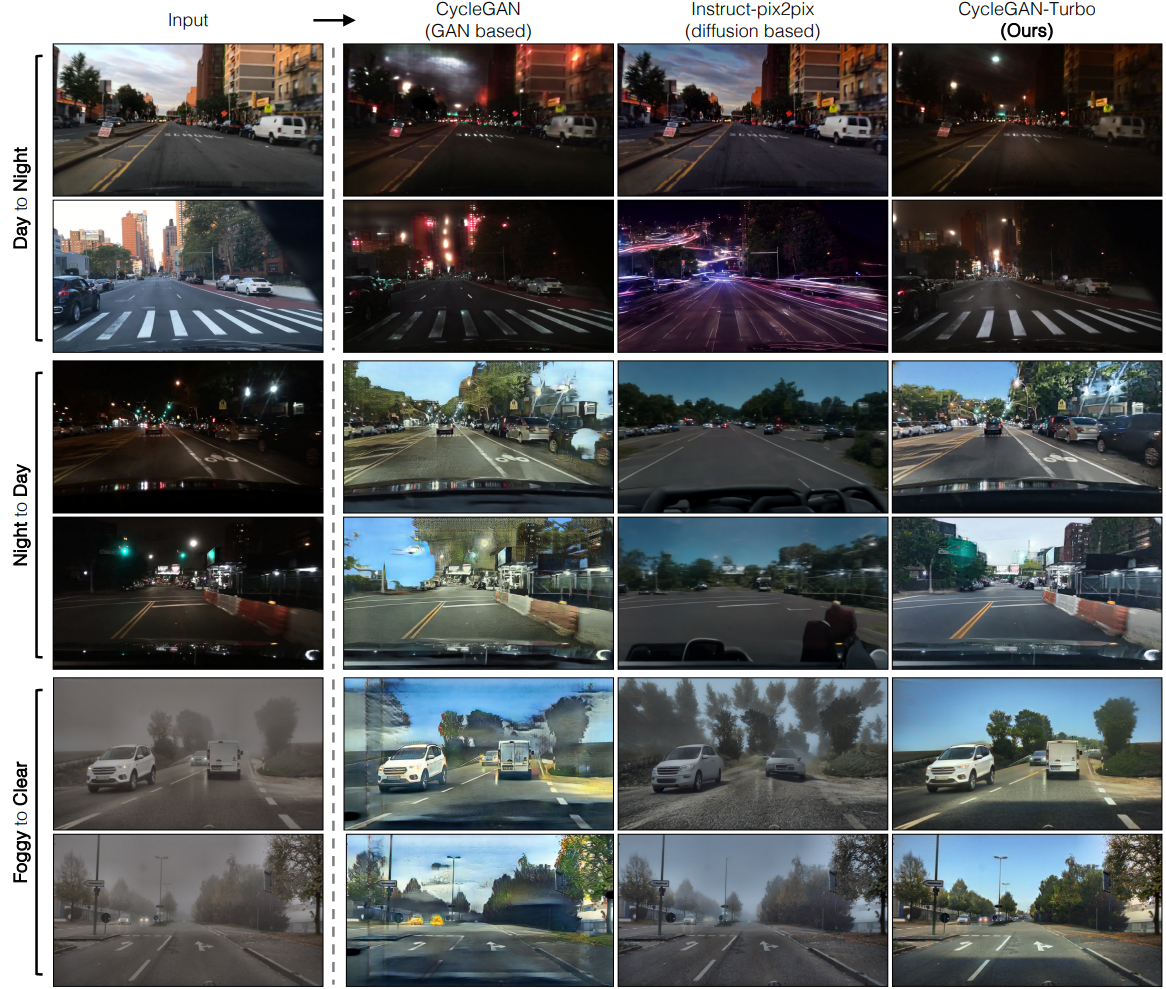
\includegraphics[width=0.5\linewidth]{images/day_night.png}
    
\end{figure}
\end{frame}
\note{   
    \begin{itemize}
        \item ähnliche Darstellung jetzt für die Tasks Day $\rightarrow$ Night und Night $\rightarrow$ Day und Foggy $\rightarrow$ Clear
        \item Von links nach rechts: Input, CycleGAN, InstructPix2Pix, CycleGAN-Turbo
    \end{itemize}

}





\begin{frame}
    \frametitle{Experiments - Paired Image Translation}
    \framesubtitle{Comparison to Unpaired Methods}

    \begin{table}
        \centering
    
        \resizebox{\linewidth}{!}{
        \begin{tabular}{l c cc cc cc cc}
            \toprule 
            \multirow{3}{*}{\textbf{Method}} 
            & \multirow{3}{*}{\textbf{\shortstack[c]{Infrence \\ time }}} 
            & \multicolumn{2}{c}{\textbf{Day $\rightarrow$ Night} }
            & \multicolumn{2}{c}{\textbf{Night $\rightarrow$ Day} }
            & \multicolumn{2}{c}{\textbf{Clear $\rightarrow$ Foggy} }
            & \multicolumn{2}{c}{\textbf{Foggy $\rightarrow$ Clear} }
            \\
    
            \cmidrule(lr){3-4} \cmidrule(lr){5-6} \cmidrule(lr){7-8} \cmidrule(lr){9-10} 
            &
            & \multirow{2}{*}{\shortstack[c]{FID $\downarrow$ }}  
            & \multirow{2}{*}{\shortstack[c]{DINO \\ Struct. $\downarrow$ }} 
    
            & \multirow{2}{*}{\shortstack[c]{FID $\downarrow$ }}  
            & \multirow{2}{*}{\shortstack[c]{DINO \\ Struct. $\downarrow$ }} 
    
            & \multirow{2}{*}{\shortstack[c]{FID $\downarrow$ }}  
            & \multirow{2}{*}{\shortstack[c]{DINO \\ Struct. $\downarrow$ }} 
    
            & \multirow{2}{*}{\shortstack[c]{FID $\downarrow$ }}  
            & \multirow{2}{*}{\shortstack[c]{DINO \\ Struct. $\downarrow$ }} 
            
            \\ \\
            \cmidrule(lr){1-10}
    
            CycleGAN \cite{zhu2020unpaired} & 0.02s
            & 36.3 & 3.6 
            & 92.3 & 4.9 
            & 153.3 & 3.6 
            & 177.3 & 3.9 
            \\
            
            CUT \cite{park2020contrastive} & 0.03s
            & 40.7 & 3.5 
            & 98.5 & 3.8
            & 152.6 & 3.4 
            & 163.9 & 4.8  \\
            
            \hdashline
    
            SDEdit \cite{meng2022sdedit} & 3.10s
            & 111.7 & 3.4 
            & 116.1 & 4.1 
            & 185.3 & 3.1
            & 209.8 & 4.7\\
    
            
            Plug\&Play \cite{tumanyan2022plugandplay} & 19.67s
            & 80.8 & 2.9 
            & 121.3 & \textbf{2.8} 
            & 179.6 & 3.6 
            & 193.5 & 3.5 \\
            
            Pix2Pix-Zero \cite{parmar2023zeroshot}  & 43.28s
            & 81.3 & 4.7 
            & 188.6 & 5.8
            & 209.3 & 5.5
            & 367.2 & 13.0
            \\
            
            Cycle-Diffusion \cite{cyclediffusion}  & 11.38s
            & 101.1 & 3.1 
            & 110.7 & 3.7 
            & 178.1 & 3.6 
            & 185.8 & 3.1\\
    
            DDIB \cite{su2022dual} & 11.93s
            & 172.6 & 9.1
            & 190.5 & 7.8 
            & 257.0 & 13.0 
            & 286.0 & 7.2  \\
    
            InstructPix2Pix \cite{brooks2023instructpix2pix} & 11.41s
            & 80.7 & \textbf{2.1} 
            & 89.4 & 6.2 
            & 170.8 & 7.6 
            & 233.9 & 4.8 
            \\
            \hdashline
    
            CycleGAN-Turbo & 0.29s
            & \textbf{31.3} & 3.0
            & \textbf{45.2} & 3.8 
            & \textbf{137.0} & \textbf{1.4}
            & \textbf{147.7} & \textbf{2.4} \\
    
            \bottomrule 
        \end{tabular}
        }
        \vspace{-18pt}
    
        \label{tab:cmp_driving_ds}
    \end{table}


\end{frame}
\note{
    \begin{itemize}
        \item Auch hier hat CycleGAN-Turbo die besten Ergebnisse in allen Tasks
        \item InstructPix2Pix und Plug\&Play haben zwar bessere DINO Scores, jedoch wesentlich schlechtere FID Scores
    \end{itemize}

}


% ---------- Ablation Study ----------
\begin{frame}
\frametitle{Experiments - Paired Image Translation}
\framesubtitle{Ablation Study}


    \begin{table}   
        \centering
        \resizebox{\linewidth}{!}{
        \begin{tabular}{l c c c | cc cc cc cc}
            \toprule 
            \multirow{3}{*}{\textbf{Method} }
            & \multirow{3}{*}{\shortstack[c]{\textbf{Input} \\ \textbf{Type} }}  
            & \multirow{3}{*}{\shortstack[c]{\textbf{Skip} }}  
            & \multirow{3}{*}{\shortstack[c]{\textbf{Pre} \\ \textbf{-trained} }}  
            & \multicolumn{2}{c}{\textbf{Horse $\rightarrow$ Zebra} }
            & \multicolumn{2}{c}{\textbf{Zebra $\rightarrow$ Horse} }
            \\
    
            \cmidrule(lr){5-6} \cmidrule(lr){7-8} \cmidrule(lr){9-10} \cmidrule(lr){11-12} 
    
            &&&& \multirow{2}{*}{\shortstack[c]{FID $\downarrow$ }}  
            & \multirow{2}{*}{\shortstack[c]{DINO \\ Struct. $\downarrow$ }} 
    
            & \multirow{2}{*}{\shortstack[c]{FID $\downarrow$ }}  
            & \multirow{2}{*}{\shortstack[c]{DINO \\ Struct. $\downarrow$ }} 
            
            \\ \\
            \cmidrule(lr){1-12}
            Conf. A & Direct Input & x & x
            & 128.6 (+214\%)  & 5.2 (+148\%)
            & 167.1 (+31\%)  & 4.6 (+156\%)
            \\
            
            Conf. B & ControlNet & x & \checkmark 
            & 41.2 (+0\%)  & 7.3 (+248\%)
            & \textbf{99.4 (-22\%)}  & 8.6 (+378\%)\\
    
            Conf. C & T2I-Adapter & x & \checkmark 
            & 55.4 (+35\%)  & 4.7 (+124\%)
            & 135.4 (+6\%) & 4.8 (+167\%)\\
            
            
            Conf. D & Direct Input & x & \checkmark
            & \textbf{40.1 (-2\%)}  & 4.4 (+110\%)
            & 116.2 (-9\%) & 3.0 (+67\%) \\
            
            
            \hdashline
            Ours & Direct Input & \checkmark & \checkmark
            & 41.0 & \textbf{2.1}
            & 127.5 & \textbf{1.8}  \\
    
            \bottomrule 
        \end{tabular}
        }
    \vspace{-10pt}
        \label{tab:ablation_study}
    \end{table}
\end{frame}
\note{
    \begin{itemize}
        \item Für diesen Vergleich mit anderen Tasks verweise auf Anhang A im Paper. Spoiler: Das Ergebniss ist vergleichbar
        \item Hier wird die Wichtigkeit der verschiedenen Komponenten des Modells untersucht
        \item Conf. A: Direkter Input, keine Pre-trained Gewichte, Gewichte random initialisiert, schlechteste Ergebnisse
        \item Conf. B, C, D nutzen verschieden Pre-trained Gewichte, Conf D hat unter denen die besten Ergebnisse
        \item Zu dieser Konfiguration werden dann Skip-Connections hinzugefügt, was die Ergebnisse nochmal verbessert
    \end{itemize}
}

\begin{frame}
    \frametitle{Experiments - unpaired Image Translation}
    \framesubtitle{Ablation Study}
    \begin{figure}
        \centering
        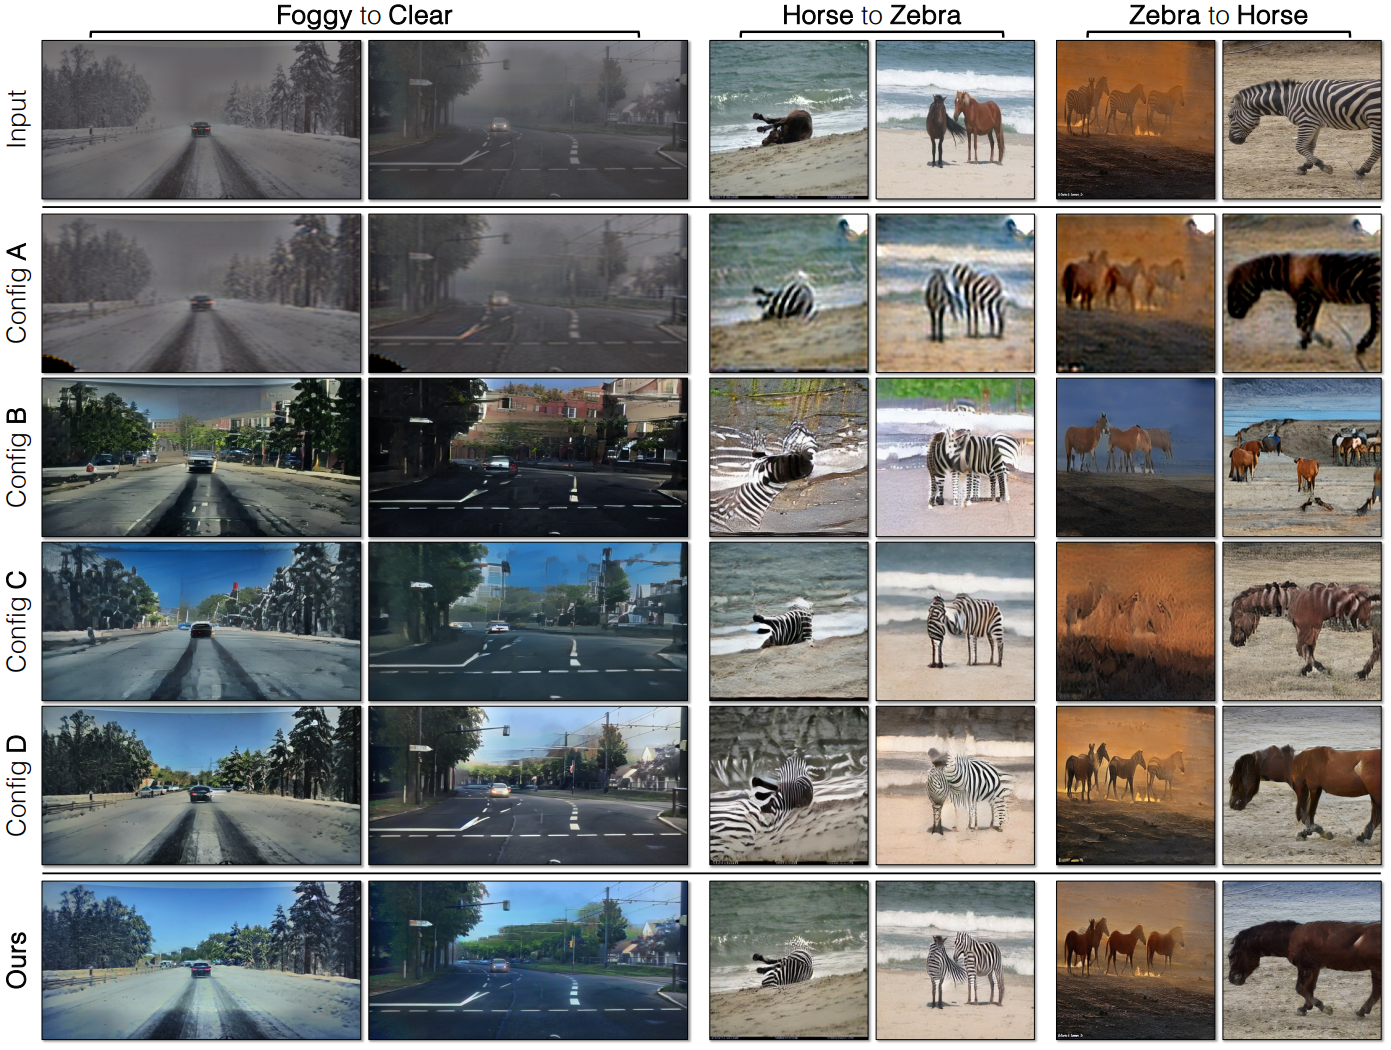
\includegraphics[width=0.55\linewidth]{images/ablation_images.png}
        
    \end{figure}
\end{frame}
\note{
    \begin{itemize}
        \item zu den jeweiligen Konfigurationen werden hier die Outputs für Horse $\rightarrow$ Zebra, Zebra $\rightarrow$ Horse und Foggy $\rightarrow$ Clear gezeigt
        \item Für die Outputs der anderen Taks verweise ich auf Anhang B im Paper
    \end{itemize}
}
% ---------- Extensions ----------
\begin{frame}
\frametitle{Experiments - Paired Image Translation}
\framesubtitle{Training Details}
\begin{block}{Loss function}
    \begin{align}
        \arg \underset{G}{\min} \mathcal{L}_{\text{rec}} + \lambda _{\text{clip}} \mathcal{L}_{\text{CLIP}} + \lambda_{\text{GAN}}\mathcal{L}_{\text{GAN}}
    \end{align}
\end{block}
with $\mathcal{L}_{\text{rec}}$ = L2-Norm + LPIPS, $\lambda_{\text{clip}} = 4$ and $\lambda_{\text{GAN}} = 0.4$
\end{frame}
\note{
    \begin{itemize}
        \item Hier wird die Loss-Funktion gezeigt, die für das Training verwendet wird
        \item $\mathcal{L}_{\text{rec}}$ Reconstruction Loss, die aus der L2-Norm und LPIPS besteht
        \item $\lambda_{\text{clip}}$ = 4
        \item $\lambda_{\text{GAN}}$ = 0.4
        \item LPIPS?
        \item CLIP?
    \end{itemize}
}

\begin{frame}
    \frametitle{Experiments - Paired Image Translation}
    \framesubtitle{Training Details}
    basiert auf Midjourney-Datensatz \footnote{https://huggingface.co/datasets/wanng/midjourney-v5-202304-clean}\\
        Edge-to-Image:
        \begin{itemize}
            \item Canny Edge Detector with random threshold
            \item Adam Optimizer with learning rate: 1e-5, batch size: 40, Steps: 7500
        \end{itemize}
        Sketch-to-Image:
        \begin{itemize}
            \item Synthetic sketches with multiple augmentations
            \item Initialized with Edge-to-Image model and fine-tuned for 5000 steps with same Optimizer
        \end{itemize}
\end{frame}
\note{
    \begin{itemize}
        \item Hier werden zwei Modelle trainiert, die auf dem Midjourney-Datensatz basieren
        \item Edge-to-Image: Hier werden mit dem Canny Edge Detector mit einem random Threshold Kanten erzeugt. \\Adam Optimizer mit Lernrate: 1e-5, Batch-Size: 40, 7500 Schritte
        \item Sketech-to-Image: Mit mehreren Augmentation werden aus den Bildern Sketches erzeugt.\\ Das Modell wird mit dem Edge-to-Image model initialisiert und dann nochmal für 5000 Schritte trainiert.
    \end{itemize}

}

\begin{frame}
    \frametitle{Experiments - Paired Image Translation}
    \framesubtitle{Comparison to Paired Methods}
    \begin{figure}
        \centering
        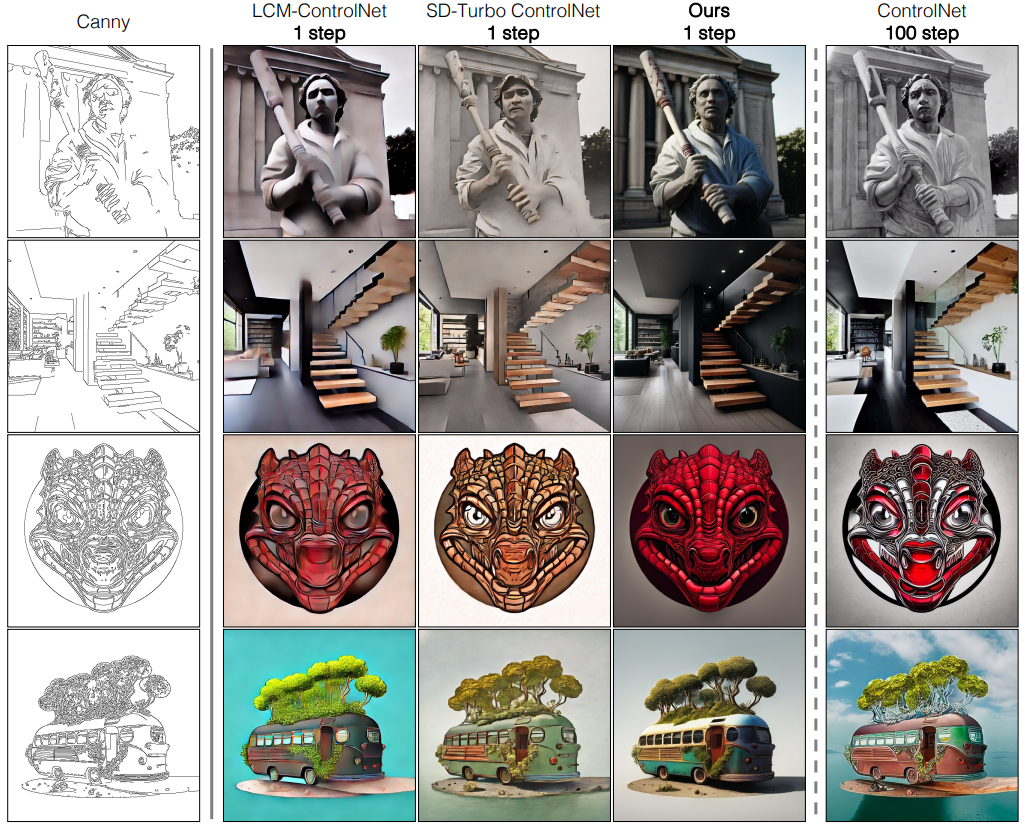
\includegraphics[width=0.5\linewidth]{images/unpaired_comp1.png}
        
    \end{figure}
\end{frame}
\note{
    \begin{itemize}
        \item Hier Edge-to-Image im Vergleich zu anderen Modellen
        \item Sichtbar mehr Realismus als die anderen Modelle
        \item Vergleichbarer Realismus zu ControlNet mit 100Schritten, obwohl das Edge-To-Image Modell 65x schneller ist
    \end{itemize}

}

\begin{frame}
    \frametitle{Experiments - Paired Image Translation}
    \framesubtitle{Comparison to Unpaired Methods}
    \begin{figure}
        \centering
        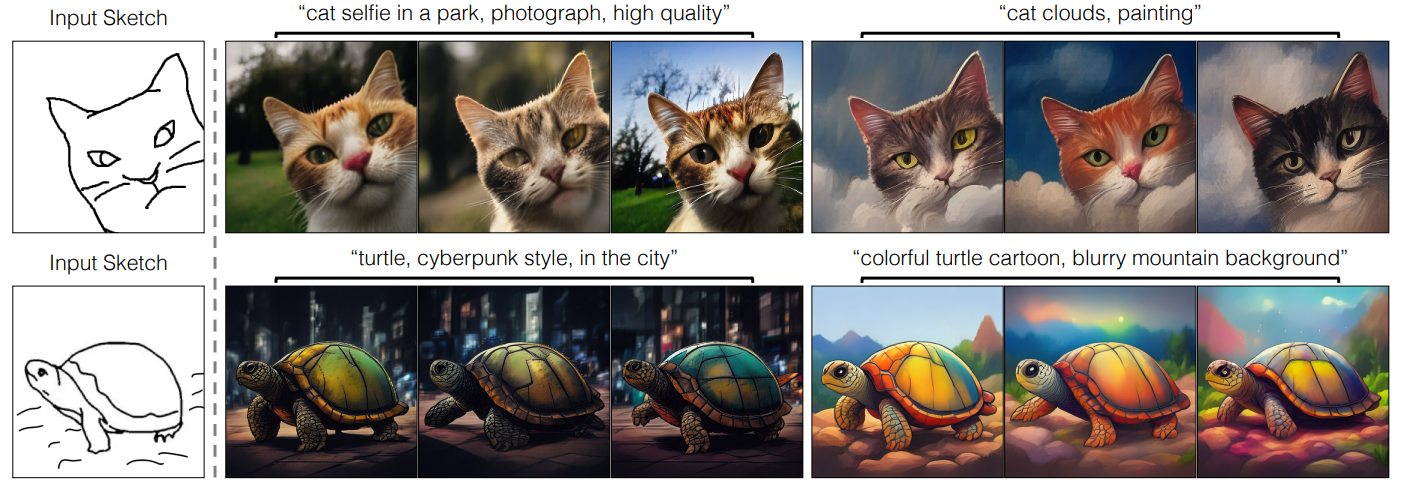
\includegraphics[width=1\linewidth]{images/unpaired_comp2.png}
            
    \end{figure}
\end{frame}
\note{
    \begin{itemize}
        \item Wie in der Methode beschrieben, ist es möglich mit dem selben Sketch und Prompt verschiedene Outputs zu generieren
    \end{itemize}
}


\begin{frame}
    \frametitle{Discussion and Limitations}
    \framesubtitle{Discussion}
    \begin{itemize}
        \item one-step pre-trained models can serve as a backbone model for many image synthesis tasks
        \item Adapting the models can be achieved through GAN objectives without multi-step diffusion training
        \item model training requires a small number of additional trainable parameters
    \end{itemize}
\end{frame}
    
% ---------- Limitations ----------
\begin{frame}
    \frametitle{Discussion and Limitations}
    \framesubtitle{Limitations}
    \begin{itemize}
        \item cannot specify strength of guidance as SD-Turbo does not use classifier-free guidance
        \item does not support negative prompt
        \item training is memory intensive
    \end{itemize}
    
\end{frame}

% ---------- End ----------
\begin{frame}
\frametitle{The End}
\begin{center}
\scalebox{2}{Questions?}
\end{center}
\end{frame}

\begin{frame}[allowframebreaks]
\frametitle{References}
\printbibliography
\end{frame}
\end{document}